\chapter{A practical take at machine learning}
\section{Modern problems}

Machine learning is based on advanced algorithms and complex data structures, performing calculations on training and validation datasets provided by the user, aswell as data received during their regular operation.

Some of the most basic models are created via techniques such as linear and non-linear regression, logistics regression or linear discriminant analysis. They result in shallow machine learning models, which have relatively small computational complexity to evaluate results of a dataset in comparison to other models \cite{shallow}.

Few of the more soffisticated methods are for example decision trees, based on algorythmical tree logic \cite{tree}. Each of the tree layer corresponds to the best predictor available at a current state, causing branching to specific values or ranges of values. The result calculation is achieved via traversing the tree from the root to one of its ending leafs. 

The most advanced, yet at the same time most demanding in complexity and memory types of models are neural networks.

Do najbardziej zaawansowanych, aczkolwiek także najbardziej wymagających obliczeniowo i pamięciowo technik uczenia maszynowego należą techniki uczenia głębokiego wykorzystujące sieci neuronowe, jak np. głębokie sieci neuronowe (ang. \textit{Deep Neural Network, DNN}) i splotowe sieci neuronowe (ang. \textit{Convolutional Neural Network, CNN}). U podstaw tych metod leży struktura sieci neuronowej, składająca się z warstwy wejściowej, jednej lub więcej warstw ukrytych posiadających neurony, oraz jednej warstwy wyjściowej. Każdy węzeł z poprzedniej warstwy połączony jest z każdym węzłem w następnej warstwie, lecz neurony znajdujące się w tej samej warstwie są wzajemnie niezależne. Każde połączenie posiada przypisaną wagę użytą do przeliczenia wartości wchodzącej do danego neuronu z danego sąsiada z poprzedniej warstwy. Wewnątrz peceptronu obliczana jest suma iloczynów wyjść z poprzednich neuronów i wag odpowiadających połączeniom, a następnie dla uzyskanej sumy obliczana jest wartość funkcji aktywacyjnej, która stanowi wartość wyjściową neuronu \cite{mit_neural}. Przykładowa sieć wykorzystująca pojedynczy neuron w pojedynczej warstwie ukrytej przedstawiona została na rys. \ref{fig:nn}. 

\begin{figure}[!ht]
    \centering
    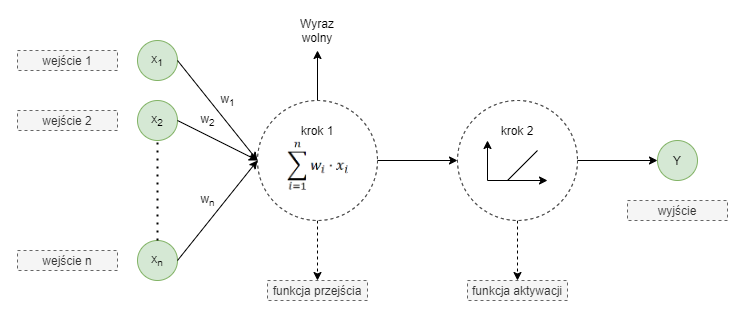
\includegraphics[width=150mm]{Rysunki/Rozdzial2/neuron.png}
    \caption{Schemat neuronu \dywiz{} Simplelearn.}
    \label{fig:nn}
\end{figure}

Bardziej rozbudowane metody wykorzystujące sieci neuronowe, jak np. CNN, wymagają dodatkowych kroków obliczeniowych związanych z wstępnym przetworzeniem danych wejściowych, aby były one przyswajalne dla wykorzystywanej sieci.

Analizując struktury danych wymagane przez poszczególne omówione powyżej rodzaje modeli, wyróżnić można następujące problemy napotykane podczas implementacji metod uczenia maszynowego \cite{constrained}:

\begin{itemize}
    \item [$\bullet$] Wymagania wydajnościowe -- są one ściśle powiązane ze złożonością obliczeniową wykorzystanych metod, wydajnością zastosowanego języka i wydajnością zastosowanej platformy sprzętowej. Docelowym efektem jest minimalizacja czasu wymaganego na uczenie modelu (chodź tutaj tolerowane są także długie czasy, szczególnie w przypadku dużych zestawów danch uczących) i czasu propagacji modelu (w przypadku czego minimalizacja czasu propagacji stanowi priorytet).
    
    \item [$\bullet$] Wymagania pamięciowe -- wynikają one z wykorzystywanych platform sprzętowych i ich ograniczeń pamięciowych. Przykładem powyższego dylematu jest zastosowanie modeli uczenia maszynowego na platformach mobilnych i platformach systemów wbudowanych, gdzie obecne rozmiary pamięci RAM i pamięci masowej (szczególnie w przypadku platform wbudowanych) potrafią być wyraźnie ograniczone w stosunku do systemów komputerowych.
\end{itemize}

W trakcie rozwoju technologii uczenia maszynowego, postawiono stanowcze kroki w kierunku rozwiązywania powyższych problemów, aby sprostać narastającym wymaganiom związanym z coraz to nowymi i bardziej skomplikowanymi zastosowaniami sztucznej inteligencji. Dokonywano tego poprzez m.in. optymalizację algorytmów, dobór platform sprzętowych o wysokim taktowaniu, możliwym zrównolegleniu operacji, oraz wykorzystaniu wysoko wydajnych języków programowania, w szczególności języków mających możliwość wykorzystania wsparcia ze strony operacji niskopoziomowych.

\section{Język C++ jako narzędzie do rozwiązania problemów uczenia maszynowego}

Dostępne są różne języki i środowiska wspierające uczenie maszynowe, począwszy od języków takich jak Python, C++, Java czy Matlab. Jednak spośród wymienionych kandydatów szczególnie istotnym wyborem jest język C++. 

C++ to język imperatywny charakteryzujący się silnym typowaniem, łączący programowanie niskopoziomowe dla konkretnych architektur z wysokopoziomowym programowaniem, w związku z czym oferuje programistom dużą kontrolę nad wykorzystaniem pamięci i możliwość optymalizacji w postaci m.in. dostosowywania wykorzystanych typów danych do wymagań funkcjonalnych tworzonej sieci, kontroli lokalizacji zmiennych (programista decyduje czy zmienna lub struktura znajdzie się na stosie czy stercie) oraz optymalizację czasów wywołań funkcji poprzez sugerowanie kompilatorowi utworzenia funkcji inline. W przeciwieństwie do języków skryptowych których kod jest interpretowany w trakcie wykonywania, takich jak Python i język środowiska Matlab, C++ jest językiem kompilowanym. Oznacza to, że program napisany w C++ przetwarzany jest z postaci tekstu do wykonawczego kodu binarnego dostosowanego do wybranej architektury procesora. Usuwa to całkowicie nadmiar złożoności obliczeniowej wykonywanego programu związanej z interpretacją poleceń i tłumaczeniem ich na język procesora danej platformy w trakcie wykonywania programu, gdyż jest to wykonywane tylko raz, na etapie kompilacji, dodatkowo pozwalając na zastosowanie przez kompilator mechanizmów optymalizacji dostępnych dla wybranej platformy \cite{cpp_char}. 

Część mechanizmów z języka C++, wywodzących się jeszcze z języka C, pozwala na wykorzystanie wstawek kodu źródłowego w języku Assembler dla wybranego procesora, co zwiększa wydajność programu kosztem przenośności kodu. Dodatkowo niektóre platformy oferują API modułów akceleracji sprzętowej (jak np. system Android udostępniający \textit{Neural Networks API, NNA} dla sieci neuronowych), co oferuje dodatkowe przyspieszenie czasu działania programu \cite{android_nna}.

\begin{figure}[!ht]
    \centering
    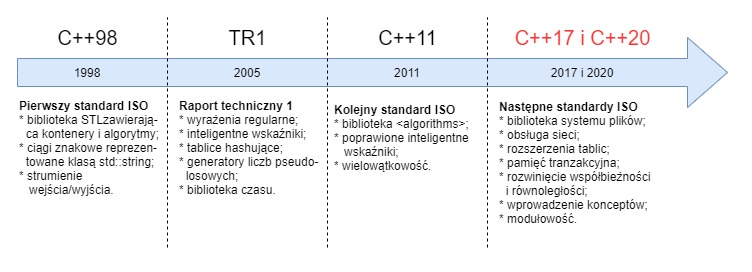
\includegraphics[width=150mm]{Rysunki/Rozdzial2/multithreading.jpg}
    \caption{Rozwój wielowątkowości w nowoczesnym C++ - Modernes C++.}
    \label{fig:cpp_history}
\end{figure}

Jedną z popularnych technik mających na celu znaczne zwiększenie wydajności modeli sztucznej inteligencji jest zrównoleglenie przetwarzania. Dostępność mechanizmów wielowątkowych dla procesorów (wprowadzonych w standardzie C++11 i dalej rozwijanych, jak przedstawiono na rys. \ref{fig:cpp_history}), oraz kompatybilność języka C++ z językiem CUDA \cite{cpp_cuda} pozwala wykonywać wiele obliczeń równolegle poprzez wykorzystanie wielu rdzeni lub oddelegowaniu części przetwarzania do karty (lub wielu kart) graficznej (gdzie liczba procesorów GPU znacząco przewyższa liczbę rdzeni CPU). Dodatkowym atutem wykorzystania języka C++ przy tworzeniu modelu sztucznej inteligencji jest łatwa integracja z programami dedykowanymi do wysokiej wydajności, napisanymi w tym języku.

Wymienione wyżej mechanizmy i cechy charakterystyczne języka umożliwiają programistom znaczną optymalizację przygotowywanych rozwiązań sztucznej inteligencji, co przekłada się na bardziej efektywne zużycie pamięci, zabezpieczenie przed przeładowaniem stosu procesora, oraz krótsze czasy propagacji utworzonych modeli.

\section{Cel powstania bibliotek}

Implementacja mechanizmów pozwalających na tworzenie rozwiązań sztucznej inteligencji, z racji na swoją złożoność, wymagania dotyczące kompetencji twórców oraz konieczność optymalizacji, jest czasochłonna i kosztowna. Tu z pomocą przychodzą biblioteki utworzone przez korporacje oraz społeczność programistów \textit{open source}. Stanowią one gotowe zbiory mechanizmów (najczęściej pisane w sposób obiektowy, a więc ubrane w klasy posiadające określone zestawy metod), które są na bieżąco optymalizowane przez grupy programistów wykorzystujące je w prywatnych projektach lub pracy zawodowej. Oferują one możliwość wykorzystania gotowych modeli utworzonych w innych technologiach, a czasem także bezpośrednie przygotowanie modelu na podstawie odpowiednio sformatowanego i odpowiednio przystosowanego zestawu danych.

Użycie gotowych bibliotek nie tylko redukuje koszty i przyspiesza tworzenie pożądanego rozwiązania sztucznej inteligencji, lecz także zapewnia większą niezawodność, gdyż elementy zawarte w bibliotece są implementowane, dokładnie testowane i poprawiane przez programistów o wysokich kompetencjach, jak m.in. w przypadku biblioteki TensorFlow posiadającej wsparcie od pracowników Google.

Większość bibliotek przeznaczonych do uczenia maszynowego, nawet wykorzystywanych w językach takich jak Python, napisana jest w języku C++, oferując API dostępne dla określonych języków docelowych. Niestety, nie wszystkie biblioteki napisane w ten sposób oferują dostęp do całego API w języku C++ dla wykorzystujących je programów zewnętrznych, lub bywa on utrudniony i skomplikowany, co sprawia że w powszechnej praktyce część bibliotek dedykowanych językowi C++ operuje na modelach przygotowanych w ramach innej, lub czasem nawet tej samej biblioteki, napisanych w innym języku. Częstym przypadkiem jest tutaj wykorzystanie właśnie języka Python do utworzenia grafu modelu lub modelu w formacie ONNX (ang. \textit{Open Neural Network Exchange}) \cite{cpp_onnx}. 

W ramach analizy porównawczej w niniejszej pracy, porównywane będą biblioteki oferujące zarówno tworzenie modeli w ramach języka C++, jak i wymagające wykorzystania modeli z innego źródła. 